
\chapter{Processor instruction set encoding}

Main contributions of this chapter are: firstly, it formulates several
instruction set encoding problems in terms of the TPG model; secondly,
it establishes that the problems can be reduced to the corresponding Boolean satisfiability (SAT) problem instances
leading to their automated solution; thirdly, it demonstrates application
of the TPG methodology at different stages of a processor design
flow --- from architectural-level specification, design and behavioural
description of an instruction set to its encoding and synthesis of
the physical implementation of the microcontroller. The chapter is organised
as follows. Section~\ref{sec:pg-encoding-problem-statement} introduces
the TPG encoding problem, overviews the existing encoding techniques and gives
a brief introduction to the new technique of globally optimal encoding.
A method for automated translation of the problems into SAT instances
is explained in Section~\ref{sec:SAT-formulation}. It is followed
by a processor design and synthesis example in Section~\ref{sec-processor} and
conclusions.

\label{chap:PGEncoding}

The chapter is based on the results published in~\cite{cpog_encoding}. It shows how to represent processor instruction sets using TPG formalism and provides
a ground for a concise formulation of several encoding problems, which
are reducible to the well-known SAT problem
and can be efficiently solved by modern SAT solvers. Application of
all the presented techniques is demonstrated on a processor design
example.

\section{Introduction\label{sec:PGEncoding-intro}}

Automated design and synthesis of both application-specific and general-purpose
instruction-set processors is an active area of research~\cite{2006_dutt_chapter}
with instruction set architecture (ISA) design seeing new techniques and improvements~\cite{2002_qin_date}.

%Automated design of general purpose processing cores, application-specific
%instruction-set processors (ASIPs), and distributed Systems-on-Chip
%(SoCs) has gained a lot of attention from academia and industry.
%New formalisms for data-path modelling are proposed~\cite{2010_mokhov_ieee}\cite{2008_sokolov_sdfs},
%hardware/software co-design methodology~\cite{1993_alomary_edac}
%is actively developed and applied for ASIP performance improvement,
%more specific techniques (such as compiler-directed instruction set
%optimisation~\cite{2002_qin_date}) are constantly introduced into
%the instruction set architecture (ISA) design domain.

Synthesis of instruction sets is a particularly active research area.
There are methods of automated derivation of ISA for a given platform
according to available system components
and for given software requirements. These methods eventually produce a
set of instructions satisfying certain properties (orthogonality,
completeness, regularity, etc.); instructions are grouped into categories
and each category is allocated a certain opcode range within the
code space~\cite{2003_nohl_dac}. At this point automation is typically
stopped or becomes trivial: the instructions are given arbitrary codes
within the allocated ranges. This limits performance due to instruction
decoder circuitry overheads. The problem is usually approached by
ad-hoc heuristics or application-specific optimisation techniques
(see, for example,~\cite{2002_lee_iccad}).

The TPG notation has an application in CPU design with a natural hardware correspondence: it describes synchronous or asynchronous control logic over the units defined by graph vertices. Such logic is commonly called a \emph{decoder} -- a circuit that takes an instruction code word and produces control signals for CPU components.

Note that the graph we are interested in when studying asynchronous control logic is the \emph{causality graph}, the graph where the nodes correspond to events (CPU component activations) and arcs correspond to causal dependencies. Causality relation is naturally transitive, and the causality graph is parameterised on code word, exactly the kind of graphs you can describe with the TPG formalism.

We are going to address the problem of TPG \emph{encoding} (related to CPOG encoding~\cite{2009_mokhov_phd}) -- the process of identification of an efficient TPG from which a given set of partial orders can be obtained via the TPG specialisation mechanism. An efficient encoding makes it possible to describe systems in
a compact functional form and apply structural synthesis methods which
significantly improve performance of the whole design flow. These
features make the model very efficient for representation and management
of processor instruction sets in hardware and EDA software. 

We discuss the known TPG encoding techniques:
\begin{itemize}
\item \emph{binary encoding}, synthesising a TPG with the minimal number of variables;
\item \emph{matrix encoding}, where each vertex and arc are assigned a unique control variable;
\item \emph{one hot enconding}, attributing a variable to each unique original scenario;
\item \emph{weakly optimal encoding}\footnote{In \cite{2009_mokhov_phd}, this is referred to simply as \emph{optimal}.} finds a solution with the minimal total number of variables among the solutions with fewest literals (ground terms); like the matrix encoding, it yields a TPG with single variable conditions; however, generally, it uses fewer variables in total.    
\end{itemize}

We proceed to discuss how we improve upon this work by introducing a new algorithm. The algorithm is able to identify a globally optimal solution for a given fixed set of optimality criteria. The techniques discussed above are only able to identify various forms of local optimums. More precisely, the four existing techniques define just four points in the \emph{solution space} constructed by our algorithm. Only one of these points is located on the Pareto optimality frontier, constructed by our algorithm (see Fig.~\ref{fig:pareto}).

\begin{figure}[t]
\centering
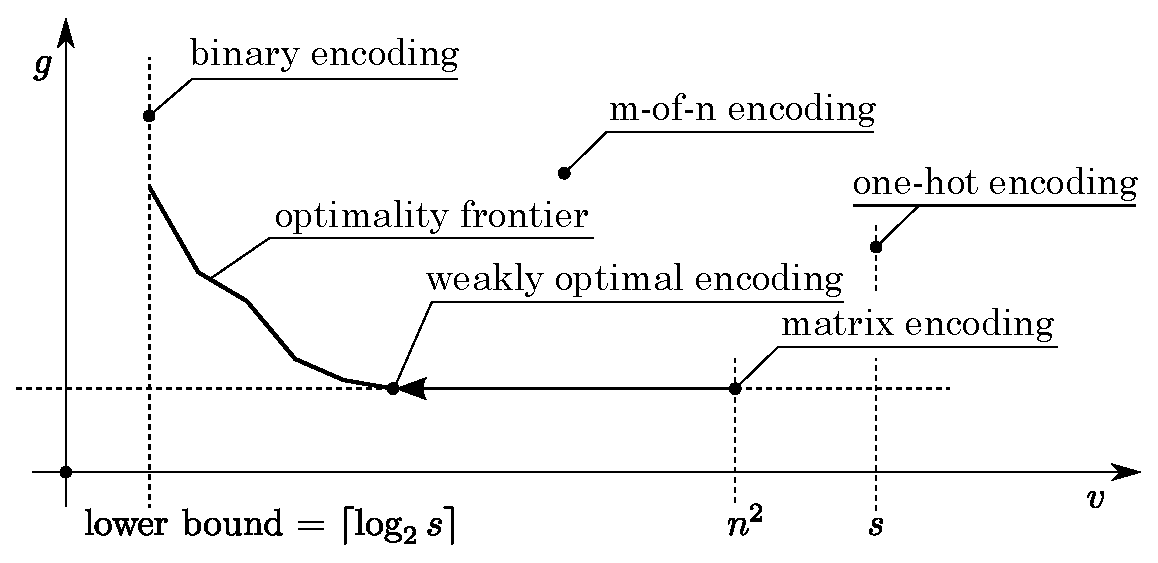
\includegraphics[scale=0.7]{fig/optimality_frontier}
\caption[The optimality frontier]{\label{fig:pareto}The relationship between the optimality frontier, as found by our algorithm, and the solutions proposed in~\cite{2009_mokhov_phd}. On the axis $g$ we plot the number of logic gates needed to describe the instruction decoder and the axis $v$ corresponds to the number of variables used to encode the instructions.}
\end{figure} 
 
The gist of the approach lies in a combination of binary search and Boolean satisfiability solving (SAT). Binary search travels through a binary tree of potential solutions using a choice function of the form $f \in D \rightarrow \mathbb{B}$ where $D$ is domain limiting the space of explored solutions. In our case, such $D$ may define either a set of gate counts of a decoder circuit or, alternatively, the set of number of variables used in TPG conditions. In a general case, $f$ takes the following form: 

$$f(x) = \left \{ \begin{array}{l} 1,~ \text{when there exists a solution} ~ S ~ \text{such that its cost is}~ x \\ 0,~ \text{otherwise}  \end{array} \right .$$   

\noindent
Such function $f$ may be challenging to compute since the set from which solutions are drawn is typically large. Let $v$ and $g$ signify the maximum number of variables and gates; also let $s$ be the number of scenarious encoded in the original TPG. Then the size of the solutions space is in the order of 

$$\left (2 (v + g) \right )^{2g} \left (2^{v} \right )^{s}$$  

\noindent For instance, for $v=5$, $g=5$ and $s=5$ the formula above gives circa $10^{21}$ potential solutions to consider. Clearly, computing $f$ with a brute-force approach is infeasible. Note, however, that $f$ has a form of an existential quantifier binding indentifiers to finite domains. This form of statement is perfectly suited for SAT solving. To bridge to the SAT-level notation we have to do binary vector encoding of scenario and variable indices, gate identifiers and cost indicators. The result is processed by a SAT solver and the output is a binary representation of a decoding circuit. In particular, we have used \noun{MiniSat}~\cite{2004_miniSAT_lncs} and \noun{clasp}~\cite{clasp} SAT solvers. As one example, we have been able to obtain an optimal solution for $v=8$, $s=8$ and $g \in 3 .. 12$.     


\section{Problem statement\label{sec:pg-encoding-problem-statement}}
In microcontroller design, the encoding of an instruction set is a common reoccuring problem. A form of encoding optimality is essential to achieve a more compact instruction decoder logic, while, at the same time, offering higher decoding performance. The first step is to represent each instruction microcode as a TPG \emph{scenario}. Such scenario is a program each instruction of each is a reference to a microcontroller unit. The directed graph semantics underlaying PGs expresses the casual dependendencies between events of unit firings; informally, this means that instruction execution steps may be ordered sequentially or concurrently.   


An encoding scheme must ensure that every scenario is adeqautely represented in the composed graph. This property, called the \emph{encoding correctness condition}, is formulated by the following statement

$$
S_i = G \mid_{X = \theta_i} 
$$

\noindent
here $X$ is the set of free variables of PG $G$ (Chapter~\ref{chap:PGAlgebra}), $S_i$ is a scenario from a scenario set $S$ and $X = \theta_i$ stands for $\bigwedge_{x \in X} \mathsf{x} = \theta_i(x)$. The condition states that a scenario is properly decoded by applying an opcode-defined graph specialisation $\theta$. Every encoding schema may be characterised by a specific choice of set $X$ and encoding function $\theta$. We refer to a tuple of $(X, \theta)$ as encoding of a scenario set $S$.


To uniquely determine, upto PG equivalence, and for encoding and scenario set a compositional graph $G$ one also needs to consider the \emph{property of composition minimality}: 

$$
G = \sum_{i < n} [X = \theta_i](G \mid_{X = \theta_i}) 
$$

\noindent
Informally, the condition states that $G$ does not contain anything in addition to the encoding of scenarios $S$.

To give an intuition behind encoding we shall consider a simple case of encoding for two scnearios $S_1, S_2$. This encoding is constructed by putting together, in a certain manner, graphs $S_1$ and $S_2$. More precisely, we overlay the graphs of $S_1$ and $S_2$ using the $+$ operator: 

$$
G \DEF [X = \theta_1]S_1 + [X = \theta_2]S_2
$$

\noindent
The overlaid graphs are conditioned by their opcodes. In the above, $\theta_1, \theta_2$ is a unique value of vector $X$ identifying a given scenario. 

In a general case, for $n$ scenarios, this statement takes the following form:

$$
G \DEF \sum_{i < n} [X = \theta_i]S_i 
$$

\noindent
Such encoding constructing preserves the property of composition mininimality provided the correctness property also holds. Let us now briefly consider one particilar encoding scheme - the \emph{one hot} encoding - to the composition of scenarios $S_1, S_2$: 

$$
G \DEF [\mathsf{x}_1 = 1 \wedge \mathsf{x}_2 = 0]S_1 + [\mathsf{x}_1 = 0 \wedge \mathsf{x}_2 = 1]S_2
$$

\noindent
It is easy to check that one hot encoding satisfies the correctness condition. For instance, for the case of scenario $S_1$, we can prove that the scenario can be obtained via graph $G$ specialisation as follows:


$$
S_1 = ([\mathsf{x}_1 = 1 \wedge \mathsf{x}_2 = 0]S_1 + [\mathsf{x}_1 = 0 \wedge \mathsf{x}_2 = 1]S_2) \mid_{\mathsf{x}_1 = 1 \wedge \mathsf{x}_2 = 0}
$$

\noindent
which is obviously correct by the definition of the specialisation operator $H|_p$.


A common measure of complexity of a Boolean formula $f$ is denoted
as $C(f)$ and is defined to be the total count of literals in it,
e.g. $C(x\cdot z+y\cdot\overline{z})=4$, $C(1)=0$, etc. 
This is the metric used in \cite{2009_mokhov_phd} to assess the produced encodings.
Indeed, when applied to a single formula this metric often works well:
the more literals the formula has, the larger the circuit to evaluate this formula.
However, when used to assess multiple similar formulae or a single formula with repeating sub-formulae,
this metric fails to account for the fact that the outputs of logic gates evaluating the subformulae
can be reused. To take advantage of this fact we use the new metric $G(C)$, showing the total number of
 gates in the circuit needed to compute all of the conditions found in $C$.
We use two versions of this metric, differing in type of gates allowed: one with AND/OR gates with 
all possible input and output inversions and another one with NAND-gates only.

\subsection{Overview}

In this section we briefly discuss the encoding approaches developed in \cite{2009_mokhov_phd}. We implement as SAT-based solution for the pre-existing techniques (weakly optimal encoding) and introduce a new, more powerful technique for identifying globally optimal solutions. 

\subsubsection{One hot}

The one hot encoding scheme associates a unique indicator variable (a hot wire) with each scenario. The set of free variables is exactly that of the scenarios being encoded:

$$
X = \mathbf{S}
$$

\noindent
where $\mathbf{S}$ is the scenario set. The encoding is very simple: one sets $i$-th bit to 1 to select an $i$-th scenario and the rest must be reset to zero:

$$\theta_i(s) = (S_i = s), \quad \text{where} ~ s, S_i \in \mathbf{S}$$


\subsubsection{Matrix encoding}

The matrix encoding allocates a unique variable for each edge and vertex of scenario graphs $S_i$. Hence, the set of free variables is given as

$$
X = \{0\}\times V \cup \{1\} \times  E
$$

\noindent
An encoding bit is set depending on whether a given edge or vertex are included in a given scenario $s$: 
 
$$
\begin{array}{l}
\theta_i(0, v) = C_i(v), \quad \text{where} ~ v \in V_i \\
\theta_i(1, e) = D_i(e), \quad \text{where} ~ e \in E_i  
\end{array}
$$

\noindent
where scenario $S_i$ is defined by a PG of the form $(V_i, E_i, C_i, D_i, X_i)$.

\subsubsection{Binary encoding}

Binary encoding associates a scenario index with the value of binary number coded by an instruction opcode. One specific form of $X$ can be given as    

$$
X = 1 .. \lceil \log | \mathbf{S} | \rceil
$$

\noindent
where $\mathbf{S}$ is the scenario set.


The encoding function computes the $k$-th bit of $i$-th scenario opcode as a binary encoding of a natural number representing the scenario index:
 
$$\theta_i(k) = \left \lfloor {i - 1 \over {2^{k-1}}} \right \rfloor ~\mathrm{mod}~2, \quad \text{where} ~ k ~ \text{is the bit position}$$

\subsubsection{Weakly optimal\label{sec:weakly-optimal-encoding}}

The optimal encoding with unconstrained code length, which we call weakly optimal encoding, tries to minimize the size of set $X$ within the universe of solutions with 1-restricted conditions. We say that a graph is 1-restricted if all the edge and vertex conditions contain at most one literal. It has been shown in \cite{2009_mokhov_phd} that the problem of computing a weakly optimal encoding is NP-complete thus barring any attempts at brute force solutions. It is challenging to give a compact characterisation of optimal encoding in the terms of free variable set $X$ and coding function $\theta$. In the continuation of the Chapter we shall give a SAT formulation of this encoding approach. 


\subsection{Globally optimal encoding\label{Sec:Generating-optimal-opcodes}}

The weakly optimal encoding method presented above generates the smallest
PG description of a set of partial orders but the number of used
variables cannot be controlled; in many practical cases it will use
more variables than is affordable under the design or technology constraints.
In this section we briefly describe a method for generating the smallest
PG given a limit on the number of variables, i.e. given the required
length of the instruction codes.

Let $L$ be the given limit on the number of variables. We generate all non-trivial
encoding constraints and try to satisfy them with opcode variables.
Only $L$ of them are free variables $X=\{x_{1},\ x_{2},\ ...,\ x_{L}\}$;
other variables $F=\{f_{1},\ f_{2},\ ...,\ f_{m}$\} are not free
--- they are expressed in terms of variables from $X\cup F$ using
Boolean binary functions, e.g. $f_{1}=x_{1}+\overline{x_{3}}$, $f_{2}=f_{1}\cdot x_{2}$,
etc. As $L$ is fixed all we have to do is to minimise the number
of non-free variables $m$. This minimisation problem requires exploration
of large search space; fortunately, it still belongs to the NP complexity
class and we can reduce it to the SAT problem: the solver has to `guess'
all the opcodes, formulae of variables in $F$, and allocation of
all variables $X\cup F$ to the non-trivial encoding constraints.


\section{SAT formulation\label{sec:SAT-formulation}}

This section presents SAT formulations of the optimal encoding problems
described in the previous section.

The Boolean satisfiability problem (SAT) is to decide whether a given
Boolean formula $F(x_{1},\ x_{2},\ \dots,\ x_{n})$ is satisfiable
or not, i.e. if it is possible to find an assignment of Boolean values
$(\alpha_{1},\ \alpha_{2},\ \dots,\ \alpha_{n})\in\{0,\ 1\}^{n}$
to the variables $(x_{1},\ x_{2},\ \dots,\ x_{n})$ which makes the
formula true: $F(\alpha_{1},\ \alpha_{2},\ \dots,\ \alpha_{n})=1$.
As SAT is a decision (not optimisation) problem, we define a cost
function and use a binary search to minimise its value by calling
the SAT solver with different cost constraints.

We have implemented all the techniques presented in this section in
an automated software tool which uses \noun{MiniSat}~\cite{2004_miniSAT_lncs} and \noun{clasp}~\cite{clasp}
as SAT solver engines. They operate on CNF (conjunctive
normal form) representations of Boolean formulae. Since our SAT-instances
are not necessarily given in CNF, we implemented their automated conversion
to CNF formulae. This conversion introduces intermediate variables
but the overall size of the obtained formula is linear with respect
to the size of the given SAT-instance.



\subsection{Weakly optimal encoding}

To solve the weakly optimal encoding problem described 
in Subsection~\ref{sec:pg-encoding-problem-statement}
we minimise the number of colours used for a conflict graph colouring.
Minimisation is performed by solving a series of instances of the
following decision problem.

Let $G=(V,\ E)$ be an extended conflict graph, where vertices $V$
correspond to encoding constraints and edges $E\subseteq V\times V$
to conflicts between them. $V$ contains both original $V_{o}=\{\mathbf{e}_{1},\ \mathbf{e}_{2},\ \dots,\ \mathbf{e}_{n}\}$
and inverted $V_{i}=\{\mathbf{\overline{\mathbf{e}}}_{1},\ \mathbf{\overline{\mathbf{e}}}_{2},\ \dots,\ \mathbf{\overline{\mathbf{e}}}_{n}\}$
constraints, such that $V=V_{o}\cup V_{i}$. The problem is to find
a colouring of $G$ which uses no more than $m$ colours.

For every pair of vertices $(\mathbf{e}_{k},\ \mathbf{\overline{\mathbf{e}}}_{k})$
we introduce a Boolean variable $p_{k}$ and an integer number $c_{k}$
whose values have to be found by the SAT solver: $p_{k}$ indicates
which of the two vertices is coloured -- if $p_{k}=1$ (resp. $p_{k}=0$)
then $\mathbf{e}_{k}$ (resp. $\overline{\mathbf{e}}_{k}$) is coloured,
while $c_{k}$ represents the colour of the chosen vertex. 

The SAT problem $\mathcal{ENCODE}$ consists of four constraints:
\[
\mathcal{ENCODE}=\mathcal{NUM}\cdot\mathcal{COL}_{oo}\cdot\mathcal{COL}_{oi}\cdot\mathcal{COL}_{ii}
\]
where $\mathcal{NUM}$ restricts colours such that $0\le c_{k}<m$.
Encoding of numbers $c_{k}$ in Boolean domain can be different, for
example, if we use binary encoding we need $\left\lceil \log_{2}m\right\rceil $
bits for each $c_{k}$. Implementation of $\mathcal{NUM}$ depends
on the chosen encoding; its general form is:
\[
\mathcal{NUM}=\prod_{1\le k\le n}(0\le c_{k})\cdot(c_{k}<m)
\]
Constraints $\mathcal{COL}$ check that adjacent vertices are assigned
different colours:
\[
\mathcal{COL}_{oo}=\prod_{(\mathbf{e}_{j},\ \mathbf{e}_{k})\in E\cap(V_{o}\times V_{o})}(p_{j}\cdot p_{k})\Rightarrow(c_{j}\neq c_{k})
\]
\[
\mathcal{COL}_{oi}=\prod_{(\mathbf{e}_{j},\ \overline{\mathbf{e}}_{k})\in E\cap(V_{o}\times V_{i})}(p_{j}\cdot\overline{p_{k}})\Rightarrow(c_{j}\neq c_{k})
\]
\[
\mathcal{COL}_{ii}=\prod_{(\overline{\mathbf{e}}_{j},\ \overline{\mathbf{e}}_{k})\in E\cap(V_{i}\times V_{i})}(\overline{p_{j}}\cdot\overline{p_{k}})\Rightarrow(c_{j}\neq c_{k})
\]
If we assume that complexity of comparison operations over numbers
$c_{k}$ is $C$, then the overall complexity of $\mathcal{ENCODE}$
is $\Theta((|V|+|E|)\cdot C)$. In particular, in case of binary encodings%
\footnote{Formula $(a<b)$ for binary numbers comparison is $(a<b)=\overline{a_{0}}\cdot b_{0}+(a_{0}=b_{0})\cdot(a'<b')$
where $a'$ and $b'$ are obtained from $a$ and $b$ by removal of
their most significant digits ($a_{0}$ and $b_{0}$); the formula
is linear with respect to the lengths of $a$ and $b$.%
} the complexity is $\Theta((|V|+|E|)\cdot\log m)$. Depending on the
chosen number encodings, there are from $\Theta(|V|\cdot\log m)$
to $\Theta(|V|\cdot m)$ free variables.

If $L$ is the minimum value of $m$ for which formula $\mathcal{ENCODE}$
is satisfiable then the optimal encoding uses $L$ variables $X=\{x_{1},\ x_{2},\ ...,\ x_{L}\}$.
Values $p_{k}$ and $c_{k}$ which satisfy the formula are used to
resolve encoding constraints $\mathbf{e}_{k}$ in the following way:
if $p_{k}=1$ then $\mathbf{e}_{k}$ is resolved by $x_{c_{k}}$,
otherwise it is resolved by $\overline{x_{c_{k}}}$.


\subsection{Globally optimal encoding}

The version of the optimal encoding problem with constrained code length
is significantly more complicated and computationally intensive. It
requires finding a set of Boolean functions of $L$ arguments (where
$L$ is the specified code length) and there are $2^{2^{L}}$ of them
-- it is impossible to explore search spaces of such magnitudes, e.g.
$2^{2^{8}}$ roughly equals to the number of atoms in the universe.
To cope with this, we reduce the search space to 2-argument Boolean
functions only. From the practical point of view this is justified
by the fact that most modern technology libraries contain only 2-
or 3-input logic gates anyway. Importantly, every complex function
can be represented as a composition of simpler ones, therefore our
approach can find any function, albeit at the cost of introducing
intermediate variables. This is similar to what actually happens during
technology mapping and logic decomposition of
functional components into hardware gates~\cite{2002_cortadella_book}\cite{1994_de_micheli_book}.

Formally, let $(\mathbf{e}_{1},\ \mathbf{e}_{2},\ \dots,\ \mathbf{e}_{n})$
be a set of encoding constraints defined in Subsection~\ref{sec:pg-encoding-problem-statement},
$S$ be the number of scenarios, and $L$ be the required code length.
We are looking for such a vector $(\psi_{1},\ \psi_{2},\ \dots,\ \psi_{S})$
of $L$-bit encodings and $n$ functions $F_{j},\ 1\le j\le n$ such
that $F_{j}(\psi_{k})=\mathbf{e}_{j}[k]$ for every scenario $1\le k\le S$
(unless $\mathbf{e}_{j}[k]$ is a don't care value).

We represent a set of functions $F$ as a combinational circuit consisting
of $G$ 2-input Boolean gates, where $G$ is the value to be minimised.
An output of the circuit can be taken directly from one of its inputs
or be produced by a gate. In addition, any output can be inverted:
\[
F_{j}(\psi)=\mathit{select}(Signals(\psi),\ \mathit{oSelector}_{j})\oplus\mathit{Inv}_{j}
\]


Here $Signals(\psi)$ is a function computing all circuit signals
including both circuit inputs (given by parameter $\psi$) and gate
outputs, $\mathit{oSelector}_{j}$ is the number indicating which
circuit signal is `connected' to the $j$-th circuit output, function
$\mathit{select(V,\ k)}$ selects $k$-th element from a given vector
$V$, and $Inv_{j}=1$ iff $j$-th circuit output is inverted. Implementation
of function $select(V,\ k)$ depends on the encoding of $k$ (we used
one-hot encoding in this case, which allows for simpler implementation).
Circuit signals are computed as follows:
\[
\begin{cases}
\mathit{Signals}(\psi) & =\mathit{Wires}_{G}(\psi)\\
\mathit{Wires}_{k}(\psi) & =\begin{cases}
\psi & \textrm{\,\,\ if}\, k=0\\
\mathit{Wires}_{k-1}(\psi)\circ\mathit{Gate}_{k}(\psi) & \textrm{\,\,\ if}\,0<k\le G
\end{cases}\\
\mathit{Gate}_{k}(\psi) & =\mathit{arg}_{1,k}(\psi)\cdot\mathit{arg}_{2,k}(\psi)\\
\mathit{arg}_{j,k}(\psi) & =select(\mathit{Wires}_{k-1}(\psi),\ \mathit{aSelector}_{j,k})\oplus\mathit{InvArg}_{j,k}
\end{cases}
\]
In other words, a set of wires is initially equal to the set of circuit
inputs $(\mathit{Wires}_{0}(\psi)=\psi)$ and then is iteratively
extended by appending $Gate_{k}$ to the previously computed set of
wires $Wires_{k-1}$. Eventually, after $G$ iterations we obtain
the set of all signals $\mathit{Signals}(\psi)=\mathit{Wires}_{G}(\psi)$.
Every $Gate_{k}$ corresponds to an AND gate with possible input inversions
(indicated by $\mathit{InvArg}_{0,k}$ and $\mathit{InvArg}_{1,k}$).
Its arguments are selected by $\mathit{aSelector}_{0,k}$ and $\mathit{aSelector}_{1,k}$
from the set of wires computed in the previous iteration. This guarantees
the absence of combinational loops.

As every signal in the circuit can be optionally inverted (by setting
$\mathit{Inv}_{j}=1$ or $\mathit{InvArg}_{j,k}=1$), the resultant
gate basis includes 8 logic gates: AND, OR, NAND, NOR, plus 4 other
gates, obtained from these by inversion of exactly one of their inputs
(they do not have commonly adopted names, apart, perhaps, from Boolean
implication $x\Rightarrow y$ which corresponds to OR($\overline{x}$,
$y$)). We have also investigated a simpler basis, consisting of only
NAND gates with no optional input inversions. The basis leads to smaller
search space and works faster, but, as expected, produces larger circuits
(see Figure~\ref{fig:Comparison-of-different} for a comparison of
two bases on a processor example). If the NAND basis is used then
free variables $\mathit{InvArg}_{j,k}$ can be dropped and the formulae
for $\mathit{Gate}_{k}(\psi)$ and $\mathit{arg}_{j,k}(\psi)$ should
be modified as follows: 
\[
\begin{cases}
\mathit{Gate}_{k}(\psi) & =\overline{\mathit{arg}_{1,k}(\psi)\cdot\mathit{arg}_{2,k}(\psi)}\\
\mathit{arg}_{j,k}(\psi) & =select(\mathit{Wires}_{k-1}(\psi),\ \mathit{aSelector}_{j,k})
\end{cases}
\]
We tried to extend the 8-gate basis by addition of gates XOR and XNOR
but on practical examples it did not bring any benefit in terms of
the number of used gates, while significantly increasing the computation
time (due to additional free variables $\mathit{IsXor_{k}}$ and more
complex $\mathit{Gate}_{k}(\psi)$ functions).

In case of the standard 8-gate basis the SAT solver has to assign
the following free variables: $\psi_{j}[k]$ ($1\le j\le S,\ 1\le k\le L$),
$Inv_{j}$ ($1\le j\le n$), $\mathit{InvArg}_{0,j}$ and $\mathit{InvArg}_{1,j}$
($1\le j\le G$). Also it has to find numbers $\mathit{oSelector}_{j}$
($1\le j\le n$), $\mathit{aSelector}_{0,j}$ and $\mathit{aSelector}_{1,j}$
($1\le j\le G$). All other variables are derived.

The SAT problem $\mathcal{ENCODE}$ consists of two constraints:
\[
\mathcal{ENCODE}=\mathcal{NUM}\cdot\mathcal{EVAL}
\]
 Constraint $\mathcal{NUM}$ restricts all the selectors to their
domains:
\begin{multline}
\mathcal{NUM}=\prod_{1\le j\le n}(1\le\mathit{oSelector}_{j})\cdot(\mathit{oSelector}_{j}\le L+G)\cdot \\ \cdot\prod_{{1\le j\le2\atop 1\le k\le G}}(1\le\mathit{aSelector}_{j,k})\cdot(\mathit{aSelector}_{j,k}<L+k)
\end{multline}
Constraint $\mathcal{EVAL}$ checks that the circuit outputs satisfy
the encoding constraints:
\[
\prod_{{1\le j\le n\atop 1\le k\le S}}(\mathbf{e}_{j}[k]\neq-)\Rightarrow(F_{j}(\psi_{k})\Leftrightarrow\mathbf{e}_{j}[k])
\]


If $G_{min}$ is the minimum value of $G$ for which formula $\mathcal{ENCODE}$
is satisfiable then the optimal encoding is obtained in vectors $\psi_{j}$
($1\le j\le S$), an encoding constraint $\mathbf{e}_{k}$ is resolved
by function $F_{j}(\psi)$, and the circuit which produces these functions
contains $G_{min}$ gates.

We tried binary and one-hot number encodings in our implementation.
In both cases the complexity of the formula is $\Theta(S\cdot G\cdot(G+L))$.
The number of free variables is $\Theta(S\cdot L+(G+n)\cdot C)$,
where $C$ is $\log(G+L)$ and $G+L$ for binary and one-hot encodings,
respectively. In practice, one-hot encoding proved to be more efficient
despite significantly larger number of free variables. This can be
explained by the fact that one-hot encoding leads to simpler constraints.


\subsection{Support for dynamic variables\label{sub:Support-for-dynamic}}

A lot of practical applications require the use of \emph{dynamic
variables}, i.e. such variables that can change their values during
execution of a partial order and affect its further execution flow~\cite{2009_mokhov_phd}.
An example of such application, a processor microcontroller, is discussed
in the next section.

Dynamic variables manifest themselves as encoding constraints with
non-constant elements, e.g. $\mathbf{e}=110y1\overline{y}$, which
means that in the fourth scenario the corresponding condition has
to evaluate to some dynamic variable $y$ and in the sixth scenario
it has to evaluate to $\overline{y}$. To compute the optimal encoding
with such non-constant constraints we have to modify the method from
the previous subsection in the following way.

Let $y$ be a dynamic variable. We generate formula $\mathcal{ENCODE}_{0}$
(resp. $\mathcal{ENCODE}_{1}$) using encoding constraints where $y$
is replaced by 0 (resp. 1). Note that the free variables in both formulae
have to be the same and we have to add $y$ into the set of circuit
inputs. Then we use the SAT solver to find an assignment that satisfies
$\mathcal{ENCODE}_{0}\cdot\mathcal{ENCODE}_{1}$. Interpretation of
the resulting assignment is the same apart from the added input signal
$y$. In case of more than one dynamic variable, the process should
be repeated for each of them. Potentially this leads to an exponential
explosion of the formula. Fortunately, the number of dynamic variables
is rather small in practice, thus the explosion is not dramatic.

It is still possible to avoid the explosion of the formula by conversion
of the problem into an instance of 2-QBF problem (a quantified Boolean
formula with two quantifiers~\cite{2004_ranjan_qbf}):
\[
\exists X\,\forall Y\ \mathcal{ENCODE}
\]
where $X$ represents the set of all free variables, and $Y$ stands
for the set of dynamic variables. However, conversion of a formula
into 2-QBF does not necessarily reduce the computation time needed
to find its satisfying assignment. Implementation of a tool based
on a 2-QBF solver is a subject of future work.

The next section demonstrates application of this technique in a processor
microcontroller design.


\section{Processor design example\label{sec-processor}}

%\subsection{Dump 2}
%This section demonstrates application of the CPOG-based methodology
to specification and synthesis of processor microcontrollers, and
discusses the results of optimal instruction encoding methods presented
in the previous section. Specification of such a complex system as
a processor starts at the architectural level which helps to deal
with the system complexity by structural abstraction~\cite{1994_de_micheli_book}.
Numerous processor architectures have emerged since fundamental von
Neumann architecture\emph{~}\cite{1946_burks_architecture} and Harvard
architecture\emph{~}\cite{1946_aiken_calculator} were proposed.
The example processor is built on the basis of Harvard architecture;
however, the method for optimal encoding of instructions presented
here is applicable to both architectures, including their
numerous derivatives.


\subsection{Architecture}

Figure~\ref{app-fig-Architecture-of-example} shows the architecture
of the example processor. Separate \emph{Program memory} and \emph{Data
memory} blocks are accessed via \emph{Instruction fetch} (IFU) and
\emph{Memory access} (MAU) operational units, respectively. The
other two operational units are: ALU and \emph{Program counter increment
unit} (PCIU). The units are controlled via request-acknowledgement
interfaces (depicted as bidirectional arrows) by \emph{Central microcontroller}
which is our primary specification and synthesis objective. 

There are four registers: general purpose registers $A$ and $B$,
\emph{Program counter} (PC) which stores address of the current
instruction in the program memory, and \emph{Instruction register}
(IR) which stores opcode of the current instruction. For the purpose
of this example the actual width of the registers (the number of bits
they can store) is not important. ALU has access to all the registers
via the register bus; MAU accesses only general purpose registers;
IFU reads opcode of the next instruction into IR given its address
in PC; PCIU is responsible for incrementing PC (moving to the next
instruction). The microcontroller has access to the opcode and ALU
\emph{flags} (information about the current state of ALU which is
used in branching instructions).


Now we have to define the set of instructions of the processor. Rather
than to list every single instruction it is easier to describe classes
of instructions with the same \emph{addressing mode}~\cite{mspmanual}
and partial order representation.

\textbf{ALU operation Rn to Rn}

An instruction from this class takes two operands stored in general
purpose registers $\{A,\ B\}$, performs an operation over them, and
writes the result back into one of them (so called \emph{register
direct addressing mode}). Examples: $\mathit{ADD\ A,\ B}$ -- addition
$A=A+B$; $\mathit{MOV\ B,\ A}$ -- assignment $B=A$. Figure~\ref{app-fig-Scenarios-of-8}(a)
shows the corresponding partial order of actions that have to be performed:
ALU works concurrently with PC increment (PCIU) and the next instruction
fetch (IFU) actions. As soon as both concurrent branches are completed,
the processor is ready to execute the next instruction. Note that
it is not important for the microcontroller which particular ALU operation
is being executed ($\mathit{ADD}$, $\mathit{MOV}$, or any other)
because the partial order of actions is not affected by this choice.
It is responsibility of ALU to detect which operation it has to perform
according to the current opcode. Therefore, it is sufficient to specify
only 8 behavioural scenarios of the microcontroller (as there are
8 classes of instructions).

\begin{figure}
\begin{centering}
\subfloat[ALU op. Rn to Rn]{

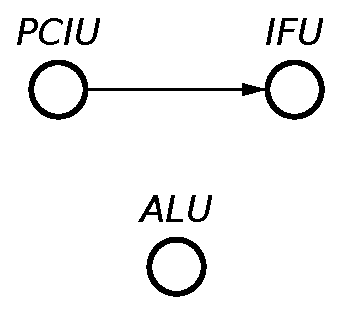
\includegraphics[scale=0.36]{fig/po_ALU_Rn_Rn}}\hfill{}\subfloat[ALU op. \#123 to Rn]{

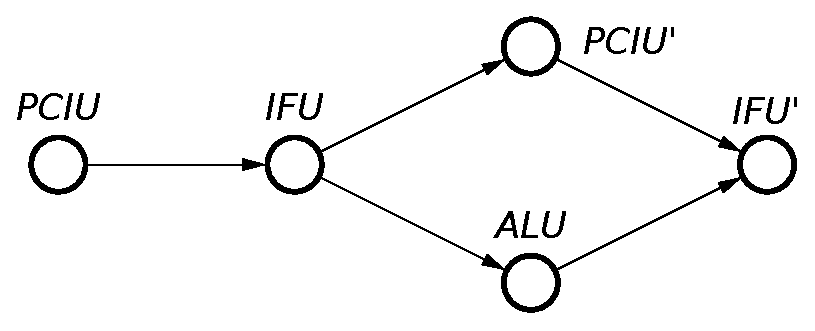
\includegraphics[scale=0.36]{fig/po_ALU_123_Rn}}\hfill{}\subfloat[ALU op. Rn to PC]{


\includegraphics[scale=0.36]{fig/po_ALU_Rn_PC}}\hfill{}\subfloat[ALU op. \#123 to PC]{

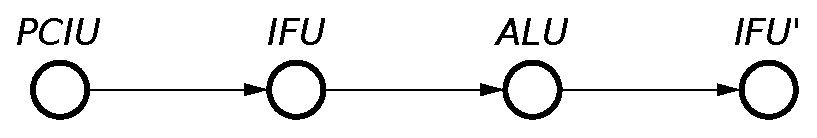
\includegraphics[scale=0.36]{fig/po_ALU_123_PC}}
\par\end{centering}

\begin{centering}
\subfloat[Memory access]{

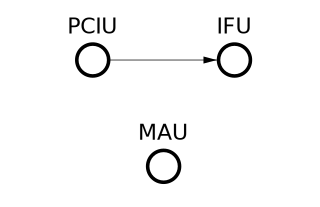
\includegraphics[scale=0.36]{fig/po_MAU}}\hfill{}\subfloat[Cond. ALU op. Rn to Rn]{

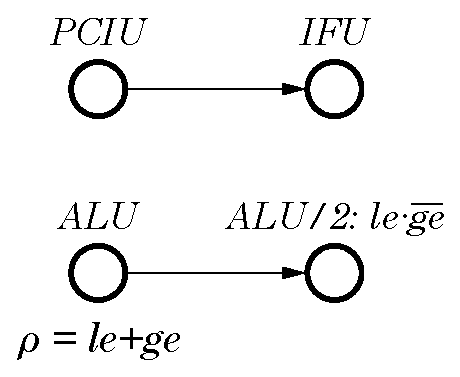
\includegraphics[scale=0.36]{fig/po_CALU_Rn_Rn}}\hfill{}\subfloat[Cond. ALU op. \#123 to Rn]{

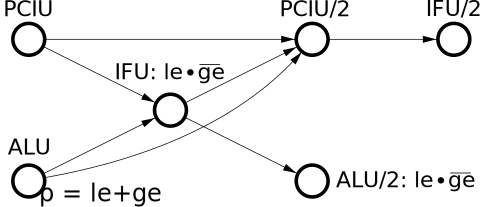
\includegraphics[scale=0.36]{fig/po_CALU_123_Rn}}\hfill{}\subfloat[Cond. ALU op. \#123 to PC]{

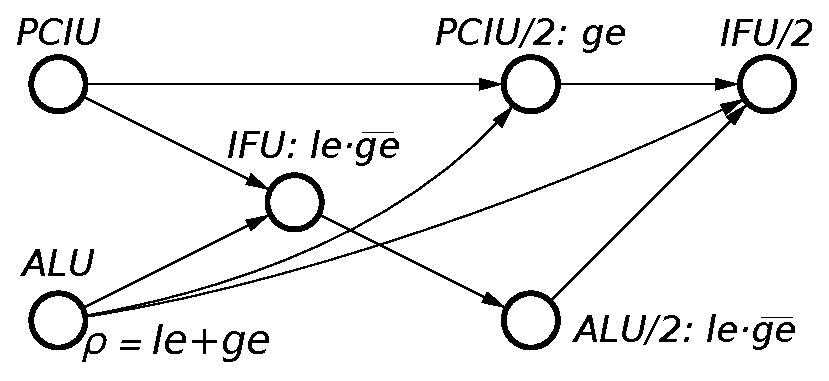
\includegraphics[scale=0.36]{fig/po_CALU_123_PC}}
\par\end{centering}

\caption{Conditional partial order specifications of 8 instruction classes\label{app-fig-Scenarios-of-8}}
\end{figure}


\textbf{ALU operation \#123 to Rn}

In this set of instructions one of the operands is register and another
is a constant which is given immediately after the instruction opcode
(e.g. $\mathit{SUB\ A,\ \#1}$ -- decrement $A$ by one), hence the
name: \emph{immediate addressing mode}. Figure~\ref{app-fig-Scenarios-of-8}(b)
shows the partial order of actions for such an instruction. At first,
the constant has to be fetched into IR (events PCIU and IFU). Then
ALU is executed concurrently with another increment of PC. Finally,
it is possible to fetch the next instruction into IR.

\textbf{ALU operation Rn to PC}

This class contains operations for unconditional branching, in which
PC register is modified. Branching can be absolute or relative: $\mathit{MOV\ PC,\ A}$
-- absolute branch to address stored in register $A$; $\mathit{ADD\ PC,\ B}$
-- relative branch to the address $B$ instructions ahead of the current
address. The partial order is very simple in this case: ALU is followed
with IFU -- see Figure~\ref{app-fig-Scenarios-of-8}(c).

\textbf{ALU operation \#123 to PC}

Instructions in this class are similar to those above with the exception
that the branch address is specified explicitly as a constant. The
actions should be scheduled in the following sequence: PCIU$\rightarrow$IFU
(to fetch the constant) followed by ALU and finally another IFU, as
shown in Figure~\ref{app-fig-Scenarios-of-8}(d).

\textbf{Memory access}

There are two instructions in this class: $\mathit{LOAD\ A}$ and
$\mathit{SAVE\ A}$. They load/save register $A$ from/to memory location
with address stored in register $B$. Figure~\ref{app-fig-Scenarios-of-8}(e)
shows that access to memory can be performed concurrently with the
next instruction fetch, exploiting the advantage of Harvard architecture.

\textbf{Conditional operations Rn to Rn, \#123 to Rn/PC}

These three classes of instructions are similar to their unconditional
versions above with the difference that they are performed only if
the following condition is true: $A<B$, i.e. register $A$ contains
a value which is less than that in register $B$. The first ALU action
compares registers $A$ and $B$, and changes ALU flags $\{le,\ ge\}$
according to the comparison result. These flags are thereafter checked
by the microcontroller in order to decide on the further scheduling
of actions. Consider, for example, conditional partial order in Figure~\ref{app-fig-Scenarios-of-8}(h).
It starts with concurrent increment of PC and comparison of registers
$A$ and $B$. If condition $A<B$ holds (i.e. $le\cdot\overline{ge}=1$)
then the process continues with the following sequence of actions:
IFU$\rightarrow$ALU/2$\rightarrow$IFU/2 (read the constant, perform
the branch, fetch the next instruction). Otherwise, the constant is
skipped (PCIU/2) and the next instruction is fetched (IFU/2). See~\cite{2009_mokhov_phd}
for details on dynamic CPOGs, which allow some of the operational
variables to be evaluated during execution of one of the scenarios
(in our case such dynamic variables are $\{le,\ ge\}$).

\begin{table}[h]
\centering

\begin{tabular}{|c||c|c|c|c|}
\hline 
\multirow{2}{*}{Instructions class} & 
\multirow{2}{*}{Trivial encoding} & 
\multicolumn{3}{c|}{ Optimal encoding} \tabularnewline
\cline{3-5}
& & $L=8$ & {$L=3$} & {$L=5$} \tabularnewline
\hline 
\hline 
{ ALU Rn to Rn} & { 000} & { 00000000} & { 000} & { 00000}\tabularnewline
\hline 
{ ALU \#123 to Rn} & { 001} & { 01001010} & { 110} & { 01001}\tabularnewline
\hline 
{ ALU Rn to PC} & { 010} & { 00010001} & { 101} & { 00010}\tabularnewline
\hline 
{ ALU \#123 to PC} & { 011} & { 01000010} & { 010} & { 01000}\tabularnewline
\hline 
{ Memory access} & { 100} & { 01000100} & { 100} & { 00100}\tabularnewline
\hline 
{ C/ALU Rn to Rn} & { 101} & { 00100000} & { 001} & { 10000}\tabularnewline
\hline 
{ C/ALU \#123 to Rn} & { 110} & { 10111010} & { 111} & { 11001}\tabularnewline
\hline 
{ C/ALU \#123 to PC} & { 111} & { 10110010} & { 011} & { 11000}\tabularnewline
\hline 
\end{tabular}

\caption{Synthesised instruction codes\label{tab:Synthesised-instruction-codes}}
\end{table}




\subsection{Processor microcontroller and instruction set design\label{app-sub-Design-of-instruction}}

This section demonstrates application of TPG-algebra to designing
processor microcontrollers. Specification of such a complex system
as a processor has to start at the architectural level, which helps
to manage the system complexity by structural abstraction~\cite{1994_de_micheli_book}.

Fig.~\ref{app-fig-Architecture-of-example} shows the architecture
of an example processor. Separate \emph{Program memory} and \emph{Data
memory} blocks are accessed via the \emph{Instruction fetch} (IFU)
and \emph{Memory access} (MAU) units, respectively. The other two
operational units are: \emph{Arithmetic logic unit} (ALU) and \emph{Program
counter increment unit} (PCIU). The units are controlled using request-acknowledgement
interfaces (depicted as bidirectional arrows) by the\textbf{\emph{
}}\emph{Central microcontroller}, which is our primary design objective. 

The processor has four registers: two general purpose registers $A$
and $B$, \emph{Program counter} (PC) storing the address of the current
instruction in the program memory, and the \emph{Instruction register}
(IR) storing the \emph{opcode} (operation code) of the current instruction.
For the purpose of this chapter, the actual width of the registers (the
number of bits they can store) is not important. ALU has access to
all the registers via the register bus; MAU has access to general
purpose registers only; IFU, given the address of the next instruction
in PC, reads its opcode into IR; and PCIU is responsible for incrementing
PC (moving to the next instruction). The microcontroller has access
to the IR and ALU \emph{flags} (information about the current state
of ALU which is used in branching instructions).

Now we define the set of instructions of the processor. Rather than
listing all the instructions, we describe classes of instructions
with the same \emph{addressing mode}~\cite{mspmanual} and the same
execution scenario. As the scenarios here are partial orders of actions,
we use TPG-algebra, and the corresponding TPGs are shown in Fig.~\ref{app-fig-Scenarios-of-8}.

\textbf{ALU operation Rn to Rn}\quad{}An instruction from this class
takes two operands stored in the general purpose registers ($A$ and
$B$), performs an operation, and writes the result back into one
of the registers (so called \emph{register direct addressing mode}).
Examples: $\mathit{ADD\ A,\ B}$ -- addition $A:=A+B$; $\mathit{MOV\ B,\ A}$
-- assignment $B:=A$. ALU works concurrently with PCIU and IFU, which
is captured by the expression $\mathit{ALU}+\mathit{PCIU\rightarrow\mathit{IFU}}$;
the corresponding PG is shown in Fig.~\ref{app-fig-Scenarios-of-8}(a).
As soon as both concurrent branches are completed, the processor is
ready to execute the next instruction. Note that it is not important
for the microcontroller which particular ALU operation is being executed
($\mathit{ADD}$, $\mathit{MOV}$, or any other instruction from this
class) because the scenario is the same from its point of view (it
is the responsibility of ALU to detect which operation it has to perform
according to the current opcode). 

\begin{figure}
\begin{centering}
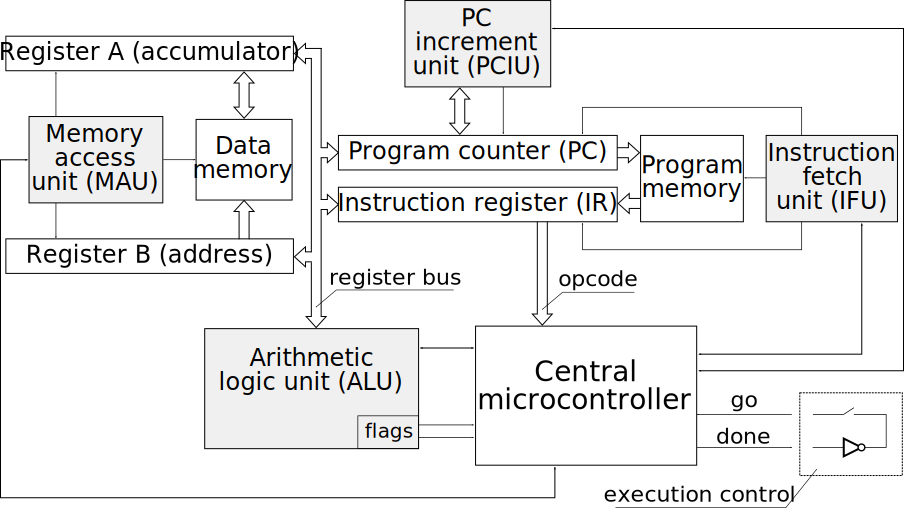
\includegraphics[width=1.04\columnwidth]{fig/processor_architecture}
\par\end{centering}

\caption{Architecture of an example processor\label{app-fig-Architecture-of-example}}
\vspace{-6mm}
\end{figure}


\begin{figure*}
\begin{centering}
\subfloat[ALU op. Rn to Rn]{

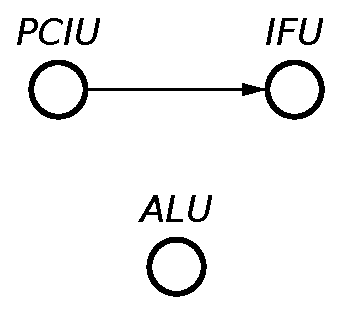
\includegraphics[scale=0.36]{fig/po_ALU_Rn_Rn}}\hfill{}\subfloat[ALU op. \#123 to Rn]{

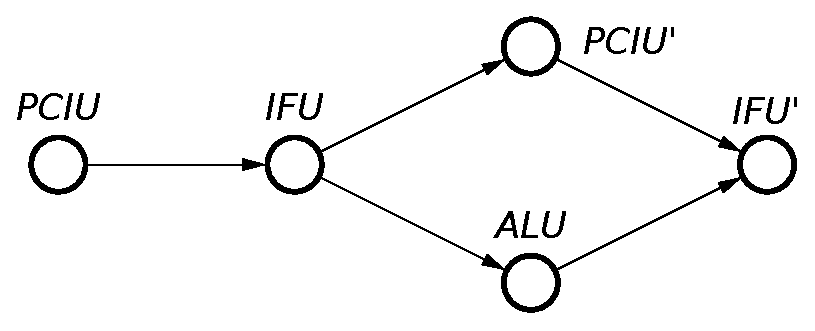
\includegraphics[scale=0.36]{fig/po_ALU_123_Rn}}\hfill{}\subfloat[ALU op. Rn to PC]{


\includegraphics[scale=0.36]{fig/po_ALU_Rn_PC}}\hfill{}\subfloat[ALU op. \#123 to PC]{

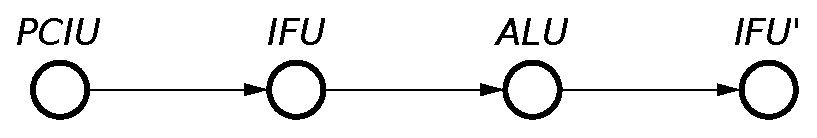
\includegraphics[scale=0.36]{fig/po_ALU_123_PC}}
\par\end{centering}

\begin{centering}
\subfloat[Memory access]{

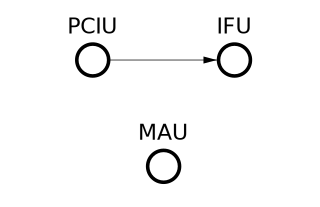
\includegraphics[scale=0.36]{fig/po_MAU}}\hfill{}\subfloat[Cond. ALU op. Rn to Rn]{

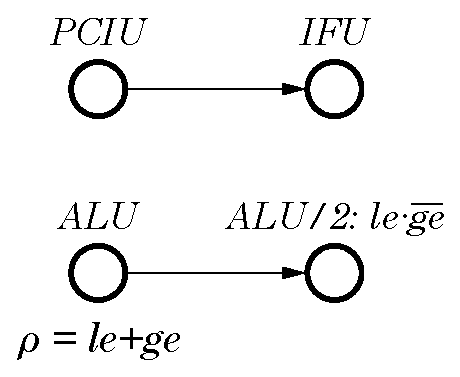
\includegraphics[scale=0.36]{fig/po_CALU_Rn_Rn}}\hfill{}\subfloat[Cond. ALU op. \#123 to Rn]{

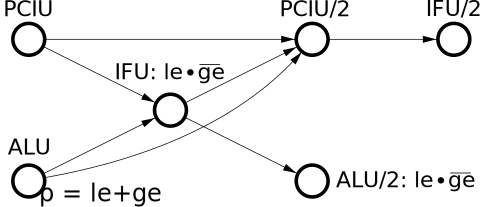
\includegraphics[scale=0.36]{fig/po_CALU_123_Rn}}\hfill{}\subfloat[Cond. ALU op. \#123 to PC]{

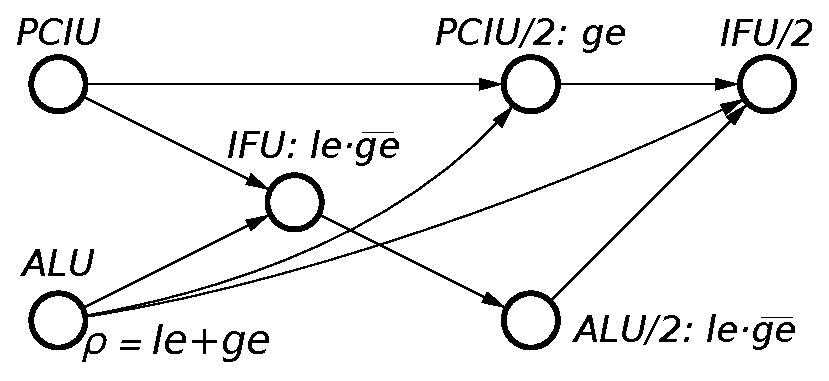
\includegraphics[scale=0.36]{fig/po_CALU_123_PC}}
\par\end{centering}

\caption{TPG specifications of instruction classes\label{app-fig-Scenarios-of-8}}
\vspace{-6mm}
\end{figure*}


\textbf{ALU operation \#123 to Rn}\quad{}In this class of instructions
one of the operands is a register and the other is a constant which
is given immediately after the instruction opcode (e.g. $\mathit{SUB\ A,\ \#5}$
-- subtraction $A:=A-5$), so called \emph{immediate addressing mode}.
At first, the constant has to be fetched into IR, modelled as $\mathit{PCIU}\rightarrow\mathit{IFU}$.
Then ALU is executed concurrently with another increment of PC: $\mathit{ALU}+\mathit{PCIU'}$
(we use $'$ to distinguish the different occurrences of actions of
the same unit). Finally, it is possible to fetch the next instruction
into IR: $\mathit{IFU'}$. The overall scenario is then $\mathit{PCIU}\rightarrow\mathit{IFU}\rightarrow(\mathit{ALU}+\mathit{PCIU'})\rightarrow\mathit{IFU'}$.

\textbf{ALU operation Rn to PC}\quad{}This class contains operations
for unconditional branching, in which PC register is modified. Branching
can be absolute or relative: $\mathit{MOV\ PC,\ A}$ -- absolute branch
to address stored in register $A$, $PC:=A$; $\mathit{ADD\ PC,\ B}$
-- relative branch to the address $B$ instructions ahead of the current
address, $PC:=PC+B$. The scenario is very simple in this case: $\mathit{ALU}\rightarrow\mathit{IFU}$.

\textbf{ALU operation \#123 to PC}\quad{}Instructions in this class
are similar to those above, with the exception that the branch address
or offset is specified explicitly as a constant. The execution scenario
is composed of : $\mathit{PCIU}\rightarrow\mathit{IFU}$ (to fetch
the constant), followed by an ALU operation, and finally by another
IFU operation, $\mathit{IFU'}$. Hence, the overall scenario is $\mathit{PCIU}\rightarrow\mathit{IFU}\rightarrow\mathit{ALU}\rightarrow\mathit{IFU'}$.

\textbf{Memory access}\quad{}There are two instructions in this class:
$\mathit{MOV\ A,\ [B]}$ and $\mathit{MOV\ [B],\ A}$. They load/save
register $A$ from/to memory location with address stored in register
$B$. Due to the presence of separate program and data memory access
blocks, this memory access can be performed concurrently with the
next instruction fetch: $\mathit{PCIU}\rightarrow\mathit{IFU}+\mathit{MAU}$.

\textbf{Conditional instructions}\quad{}These three classes of instructions
are similar to their unconditional versions above with the difference
that they are performed only if the condition $A<B$ holds. The first
ALU action compares registers $A$ and $B$, setting the ALU flag
$lt$ (less than) according to the result of the comparison. This
flag is then checked by the microcontroller in order to decide on
the further scheduling of actions. 

\textbf{Rn~to~Rn}\quad{}This instruction conditionally performs
an ALU operation with the registers (if the condition does not hold,
the instruction has no effect, except changing the ALU flags). The
operation starts with an ALU operation comparing $A$ with $B$; depending
on the result of this comparison, i.e. the status of the flag $lt$,
the second ALU operation may be performed. This is captured by the
expression $\mathit{ALU}\rightarrow[lt]\mathit{ALU'}$. Concurrently
with this, the next instruction is fetched: $\mathit{PCIU}\rightarrow\mathit{IFU}$.
Hence, the overall scenario is $\mathit{PCIU}\rightarrow\mathit{IFU}+\mathit{ALU}\rightarrow[lt]\mathit{ALU'}$.

\textbf{\#123~to~Rn}\quad{}This instruction conditionally performs
an ALU operation with a register and a constant which is given immediately
after the instruction opcode (if the condition does not hold, the
instruction has no effect, except changing the ALU flags). We consider
the two possible scenarios:
\begin{itemize}
\item $A<B$ holds: First, ALU compares $A$ and $B$ concurrently with
a PC increment; since $A<B$ holds, the ALU sets flag $lt$ and the
constant is fetched to the instruction register: $(\mathit{ALU}+\mathit{PCIU})\rightarrow\mathit{IFU}$.
After that PC has to be incremented again, $\mathit{PCIU'}$, and
ALU performs the operation, $\mathit{ALU'}$. Finally, the next instruction
is fetched (it cannot be fetched concurrently with $\mathit{ALU'}$
as ALU is using the constant in IR): $(\mathit{ALU'}+\mathit{PCIU'})\rightarrow\mathit{IFU'}$.
\item $A<B$ does not hold: First, ALU compares $A$ and $B$ concurrently
with a PC increment; since $A<B$ does not hold, the ALU resets flag
$lt$ and the constant that follows the instruction opcode is skipped
by incrementing the PC: $(\mathit{ALU}+\mathit{PCIU})\rightarrow\mathit{PCIU'}$.
Finally, the next instruction is fetched: $\mathit{IFU'}$.
\end{itemize}
\begin{figure*}
\centering{}\hspace*{\fill}%
\begin{tabular}{||c||||c||}
\hline 
{\small Instructions class} & {\small Opcode: $xyz$}\tabularnewline
\hline 
\hline 
{\small ALU Rn to Rn} & {\small 000}\tabularnewline
\hline 
{\small ALU \#123 to Rn} & {\small 110}\tabularnewline
\hline 
{\small ALU Rn to PC} & {\small 101}\tabularnewline
\hline 
{\small ALU \#123 to PC} & {\small 010}\tabularnewline
\hline 
{\small Memory access} & {\small 100}\tabularnewline
\hline 
{\small C/ALU Rn to Rn} & {\small 001}\tabularnewline
\hline 
{\small C/ALU \#123 to Rn} & {\small 111}\tabularnewline
\hline 
{\small C/ALU \#123 to PC} & {\small 011}\tabularnewline
\hline 
\end{tabular}\hspace*{\fill}\raisebox{-5em}[0em]{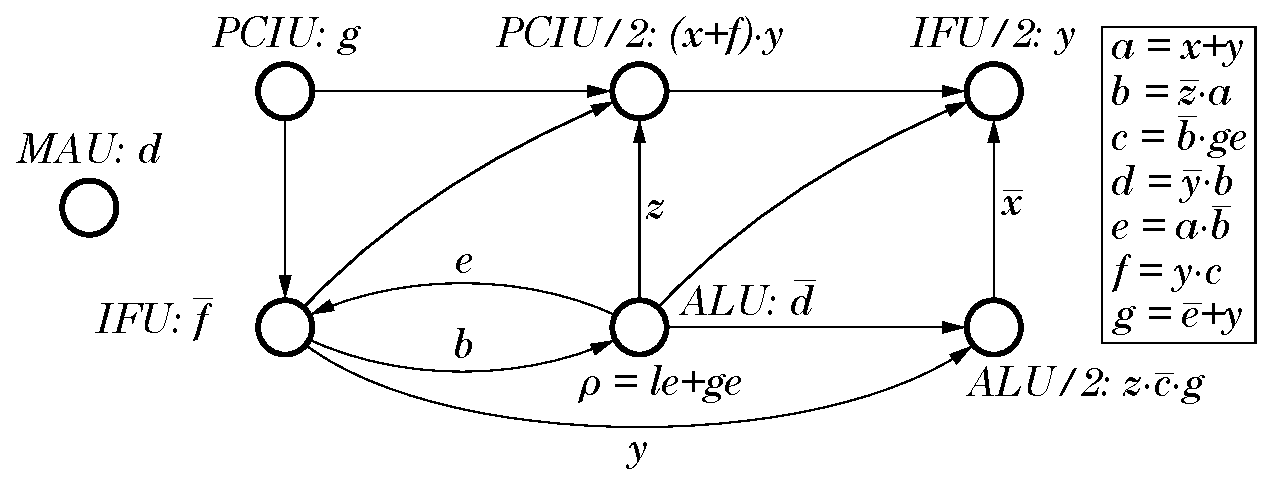
\includegraphics[scale=0.5]{fig/CPOG_L_3}}\hspace*{\fill}\caption{Optimal 3-bit instruction opcodes and the corresponding TPG specification
of the microcontroller\label{fig:opcodes-and-CG}}
\vspace{-6mm}
\end{figure*}


Hence, the overall scenario is the overlay of the two subscenarios
above prefixed with appropriate conditions (here we denote the predicate
$A<B$ by $lt$): 
\[
\begin{array}{c}
[lt]((\mathit{ALU}+\mathit{PCIU})\!\rightarrow\!\mathit{IFU}\!\rightarrow\!(\mathit{ALU'}+\mathit{PCIU'})\!\rightarrow\!\mathit{IFU'})+\\
+[\overline{lt}]((\mathit{ALU}+\mathit{PCIU})\!\rightarrow\!\mathit{PCIU'}\!\rightarrow\!\mathit{IFU'}).
\end{array}
\]
This expression can be simplified using the rules of TPG-algebra:%
\footnote{This case illustrates the advantage of using the new hierarchical
approach that allows to specify the system as a composition of scenarios
and formally manipulate them in an algebraic fashion. In the previous
paper~\cite{2011_mokhov_iet} the CPOG for this class of instruction
was designed monolithically, and because of this the arc between $\mathit{ALU'}$
and $\mathit{IFU'}$ was missed. Adding this arc not only fixes the
dangerous race between these two blocks, but also leads to a smaller
microcontroller due to the additional similarity between TPGs for
this class of instructions and for the one described below.%
}
\[
(\mathit{ALU}+\mathit{PCIU})\!\rightarrow\![lt]\mathit{IFU}\!\rightarrow\!(\mathit{PCIU'}+[lt]\mathit{ALU'})\!\rightarrow\!\mathit{IFU'}.
\]


\textbf{\#123~to~PC}\quad{}This instruction performs a conditional
branching in which the branch address or offset is specified explicitly
as a constant. We consider the two possible scenarios:
\begin{itemize}
\item $A<B$ holds: First, ALU compares $A$ and $B$ concurrently with
a PC increment; since $A<B$ holds, the ALU sets flag $lt$ and the
constant is fetched to the instruction register: $(\mathit{ALU}+\mathit{PCIU})\rightarrow\mathit{IFU}$.
After that ALU performs the branching operation by modifying PC, $\mathit{ALU'}$.
After PC is changed, the next instruction is fetched, $\mathit{IFU'}$.
\item $A<B$ does not hold: the scenario is exactly the same as in the \textbf{\#123~to~Rn
}case when $A<B$ does not hold.
\end{itemize}
Hence, the overall scenario is the overlay of the two subscenarios
above prefixed with appropriate conditions (here we denote the predicate
$A<B$ by $lt$): 
\[
\begin{array}{c}
[lt]((\mathit{ALU}+\mathit{PCIU})\!\rightarrow\!\mathit{IFU}\!\rightarrow\!\mathit{ALU'}\!\rightarrow\!\mathit{IFU'})+\\
+[\overline{lt}]((\mathit{ALU}+\mathit{PCIU})\!\rightarrow\!\mathit{PCIU'}\!\rightarrow\!\mathit{IFU'}).
\end{array}
\]
This expression can be simplified using the rules of TPG-algebra:
\[
(\mathit{ALU}+\mathit{PCIU})\!\rightarrow\!([\overline{lt}]\mathit{PCIU'}+[lt](\mathit{IFU}\!\rightarrow\!\mathit{ALU'}))\!\rightarrow\!\mathit{IFU'}.
\]


The overall specification of the microcontroller can now be obtained
by prefixing the scenarios with appropriate conditions and overlaying
them. These conditions can be naturally derived from the instruction
opcodes. The opcodes can be either imposed externally or chosen with
the view to optimise the microcontroller. In the latter case, TPG-algebra
and TPGs allow for a formal statement of this optimisation problem
and aid in its solving; in particular, the sizes of the TPG-algebra
expression or TPG are useful measures of microcontroller complexity
(there is a compositional translation from a TPG-algebra expression
into a linear-size circuit). The details on the method to select the optimal encoding
are presented in Chapter~\ref{chap:PGEncoding}.
We just note that it is natural to use three bits for opcodes as there
are eight classes of instructions, and give an example of optimal
3-bit encoding in the table in Fig.~\ref{fig:opcodes-and-CG}; the
TPG specification of the corresponding microcontroller is shown in
the right part of this figure (the TPG-algebra expression is not shown
because of its size).



\subsection{Instructions encoding}

\begin{table}[t]
\centering

\begin{tabular}{|c||c|c|c|c|}
\hline 
\multirow{2}{*}{Instructions class} & 
\multirow{2}{*}{Trivial encoding} & 
\multicolumn{3}{c|}{ Optimal encoding} \tabularnewline
\cline{3-5}
& & $L=8$ & {$L=3$} & {$L=5$} \tabularnewline
\hline 
\hline 
{ ALU Rn to Rn} & { 000} & { 00000000} & { 000} & { 00000}\tabularnewline
\hline 
{ ALU \#123 to Rn} & { 001} & { 01001010} & { 110} & { 01001}\tabularnewline
\hline 
{ ALU Rn to PC} & { 010} & { 00010001} & { 101} & { 00010}\tabularnewline
\hline 
{ ALU \#123 to PC} & { 011} & { 01000010} & { 010} & { 01000}\tabularnewline
\hline 
{ Memory access} & { 100} & { 01000100} & { 100} & { 00100}\tabularnewline
\hline 
{ C/ALU Rn to Rn} & { 101} & { 00100000} & { 001} & { 10000}\tabularnewline
\hline 
{ C/ALU \#123 to Rn} & { 110} & { 10111010} & { 111} & { 11001}\tabularnewline
\hline 
{ C/ALU \#123 to PC} & { 111} & { 10110010} & { 011} & { 11000}\tabularnewline
\hline 
\end{tabular}

\caption{Synthesised instruction codes\label{tab:Synthesised-instruction-codes}}
\end{table}

Now the instructions have to be encoded. The simplest way to do this
is to use the binary encoding scheme, i.e. assign opcodes $\{000,\ \dots,\ 111\}$
to the instructions in arbitrary order as shown in Table~\ref{tab:Synthesised-instruction-codes}
(column `Trivial encoding'). This is not optimal in terms of area
and latency of the final microcontroller implementation. To obtain
the smallest possible TPG specification one has to apply the optimal
encoding procedure from Subsection~\ref{sec:weakly-optimal-encoding}. Generated
opcodes have 8 bits instead of 3 (shown in column `Optimal encoding'
of the same table). Whether 8 bit opcodes are affordable or not depends
on the chosen width of instruction register IR and other design parameters.
If it is not possible to use 8 bit opcodes one can try to apply the
constrained synthesis problem from Subsection~\ref{Sec:Generating-optimal-opcodes}
and generate instruction codes of required length $3\le L<8$ (it
is not possible to use less than 3 bits, and there is no sense in
setting $L\ge8$ because the optimal encoding uses 8 bits). We show
the generated opcodes for cases $L=3$ and $L=5$ -- see the corresponding
columns of Table~\ref{tab:Synthesised-instruction-codes}. Note that
the optimal 3-bit opcodes are very different from the trivial $000-111$
sequential encoding.

\begin{figure}[!t]
\begin{centering}
\subfloat[Trivial encoding (35 literals)]{

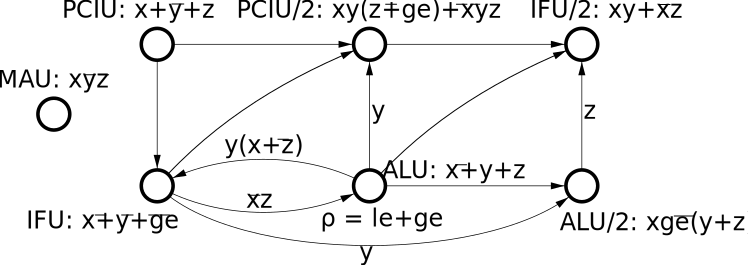
\includegraphics[scale=0.45]{fig/processor_cpog}}\hfill{}\subfloat[Optimal encoding (16 literals)]{

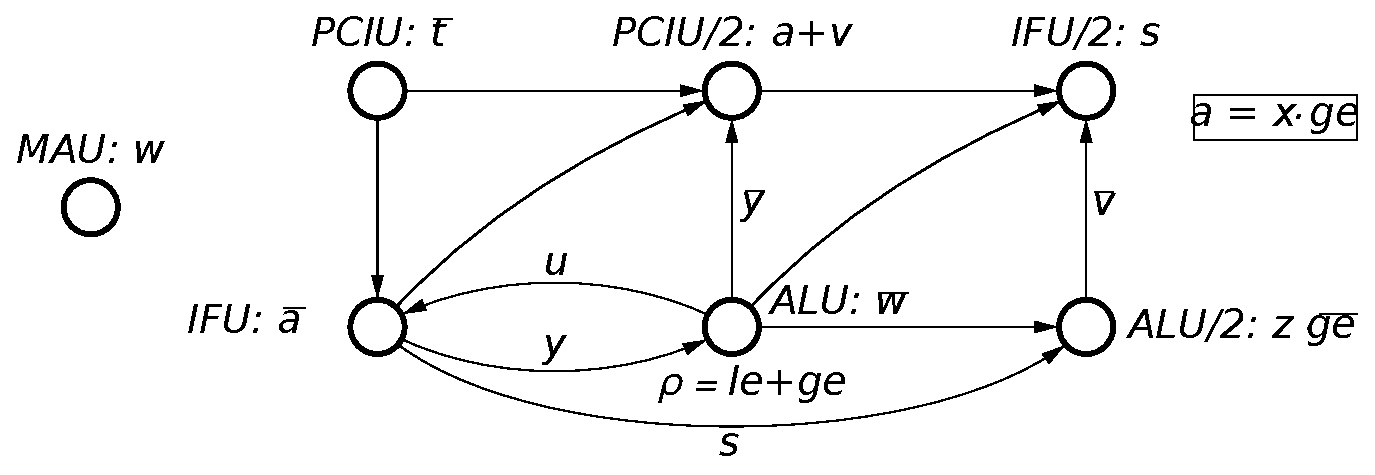
\includegraphics[scale=0.45]{fig/CPOG_L_8}}
\par\end{centering}

\begin{centering}
\subfloat[Optimal encoding $L=3$ (31 literals)]{

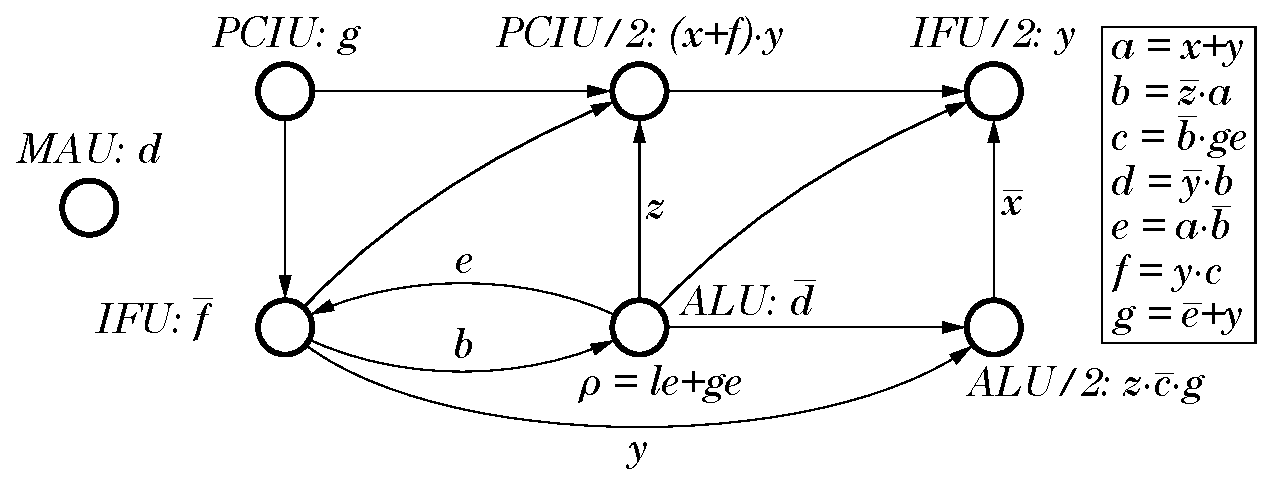
\includegraphics[scale=0.45]{fig/CPOG_L_3}}\hfill{}\subfloat[Optimal encoding $L=5$ (21 literals)]{

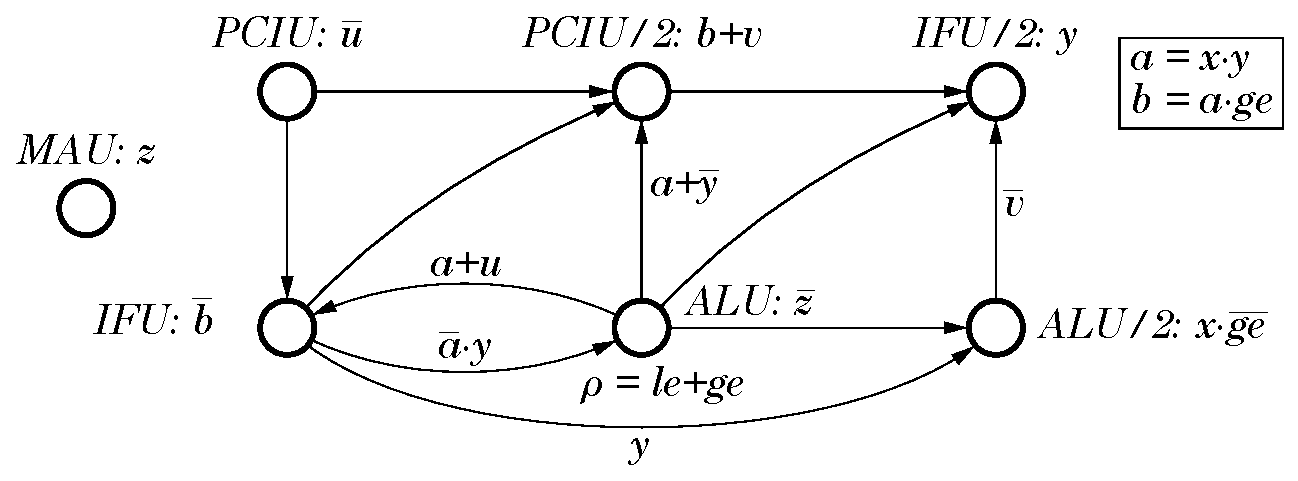
\includegraphics[scale=0.45]{fig/CPOG_L_5}}
\par\end{centering}

\caption{Synthesised CPOGs\label{fig:Synthesised-CPOGs}}
\end{figure}



\subsection{Microcontroller synthesis\label{app-sub-Microcontroller-synthesis}}

Figure~\ref{fig:Synthesised-CPOGs} shows four CPOGs obtained using
instruction encodings shown in Table~\ref{tab:Synthesised-instruction-codes}.
The trivial encoding results in the most complex CPOG shown in Figure~\ref{fig:Synthesised-CPOGs}(a);
it uses three variables $X=\{x,\ y,\ z\}$ and contains 35 literals.
The optimal encoding produces the CPOG with only 16 literals in its
conditions, Figure~\ref{fig:Synthesised-CPOGs}(b), but it uses 8
opcode variables $X=\{x,\ y,\ z,\ u,\ v,\ w,\ s,\ t\}$. Figures~\ref{fig:Synthesised-CPOGs}(c,
d) show the optimal CPOGs encoded with 3 and 5 ($X=\{x,\ y,\ z,\ u,\ v\}$)
variables, respectively; derived variables (denoted by names starting
from $a$) are shown in boxes.

\begin{figure}[!t]
\begin{centering}
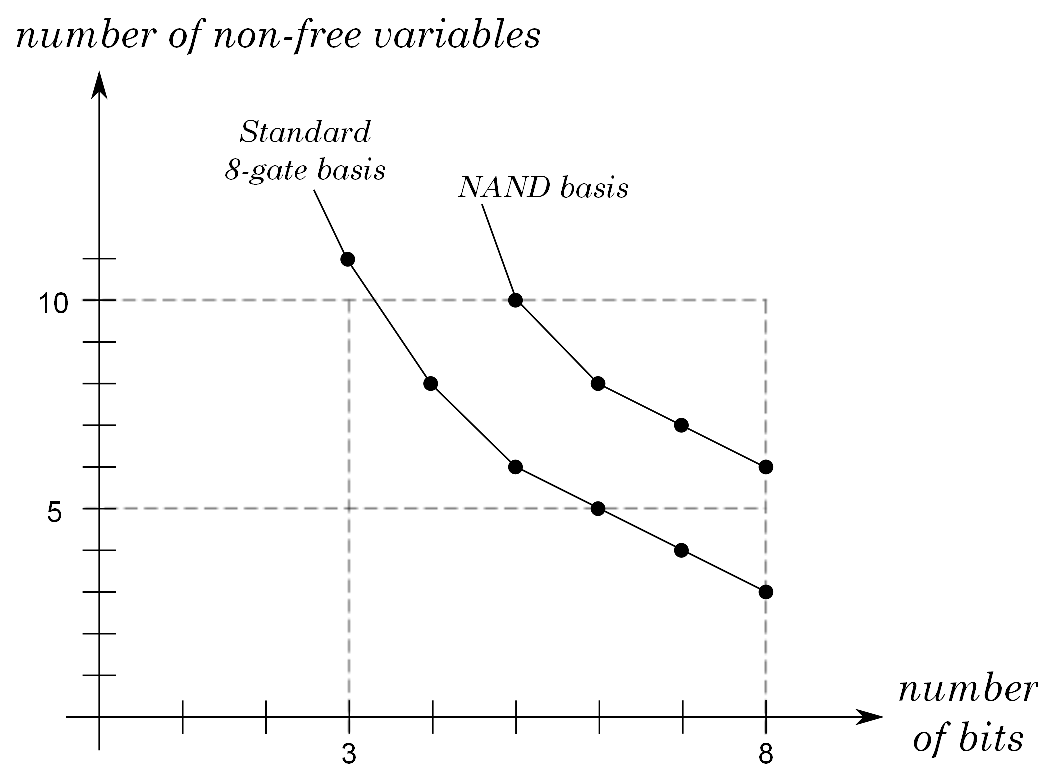
\includegraphics[scale=0.52]{fig/encoding_graph}
\par\end{centering}

\caption{Comparison of different gate bases\label{fig:Comparison-of-different}}
\end{figure}


Figure~\ref{fig:Comparison-of-different} illustrates dependency
of the number of non-free variables on the number of free variables.
As expected, the more free variables we have, the less non-free variables
are needed to satisfy all the encoding constraints. It is interesting
to note that if we restrict our functional basis to NAND gates only
(i.e. if we allow only functions $f_{k}=\overline{f_{i}\cdot f_{j}}$
to be used), the number of non-free variables does not increase dramatically.

Choice of a particular scenario within every CPOG in Figure~\ref{fig:Synthesised-CPOGs}
is highly distributed: every condition is responsible for rendering
only a little portion of the global picture and has a large don't
care set which leads to efficient Boolean minimisation. Note that
flag $le$ turned out to be redundant and was removed from all the
conditions, because original condition $le\cdot\overline{ge}$ is
equivalent to $\overline{ge}$ if the restriction function of ALU
($\rho_{ALU}=le+ge$) is satisfied: $\overline{ge}\cdot(le+ge)\Leftrightarrow le\cdot\overline{ge}$.
Thus it is enough to test only one ALU flag $ge$ to correctly schedule
all the instructions.

\begin{table}[b]
\begin{centering}
\begin{tabular}{|c||c|c|c||c|c|c|}
\hline 
Instructions class & $x$ & $z$ & $v$ & $\phi_{IFU}$ & $\phi_{ALU/2}$ & $\phi_{PCIU/2}$\tabularnewline
\hline 
\hline 
ALU Rn to Rn & 0 & 0 & 0 & 1 & 0 & 0\tabularnewline
\hline 
ALU \#123 to Rn & 0 & 0 & 1 & 1 & 0 & 1\tabularnewline
\hline 
ALU Rn to PC & 0 & 0 & 0 & 1 & 0 & 0\tabularnewline
\hline 
ALU \#123 to PC & 0 & 0 & 0 & 1 & 0 & 0\tabularnewline
\hline 
Memory access & 0 & 0 & 0 & 1 & 0 & 0\tabularnewline
\hline 
Cond. ALU Rn to Rn & 0 & 1 & 0 & 1 & $\overline{ge}$ & 0\tabularnewline
\hline 
Cond. ALU \#123 to Rn & 1 & 1 & 1 & $\overline{ge}$ & $\overline{ge}$ & 1\tabularnewline
\hline 
Cond. ALU \#123 to PC & 1 & 1 & 0 & $\overline{ge}$ & $\overline{ge}$ & $ge$\tabularnewline
\hline 
\hline 
Optimal condition & \multicolumn{3}{c|}{} & $\overline{x\cdot ge}$ & $z\cdot\overline{ge}$ & $x\cdot ge+v$\tabularnewline
\hline 
\end{tabular}
\par\end{centering}

\caption{Encoding of conditions with dynamic variable $ge$\label{app-tab-Encoding-of-non}}
\end{table}


The optimal CPOG (Figure~\ref{fig:Synthesised-CPOGs}(b)) contains
only 16 literals which leads to a twice smaller and faster microcontroller
than the one obtained using the trivial encoding. Note that in this
case it is not possible to reduce the final result to pure 1-restricted
form: the graph contains conditions depending on flag $ge$ which
cannot be mixed with other variables for optimisation purposes as
it is provided by ALU and can be changed during execution of an ALU
operation. Three non 1-restricted conditions are: $\phi(IFU)=\overline{a}=\overline{x\cdot ge}$,
$\phi(ALU/2)=z\cdot\overline{ge}$, and $\phi(PCIU/2)=a+v=x\cdot ge+v$.
It is impossible to use fewer literals for these conditions; this
is clarified in Table~\ref{app-tab-Encoding-of-non}: depending on
the instruction $\phi(IFU)$ has to evaluate either to $1$ or to
$\overline{ge}$ and this choice is delegated to operational variable
$x$ such that $\phi(IFU)=\overline{x\cdot ge}$. Condition $\phi(ALU/2)$
is similar: it must evaluate either to $0$ or to $\overline{ge}$,
hence $\phi(ALU/2)=z\cdot\overline{ge}$. The most complicated case
is presented with condition $\phi(PCIU/2)$ which has three possible
evaluations: $0$, $1$, and $ge$. Two variables are needed to handle
this leading to $\phi(PCIU/2)=x\cdot ge+v$. Optimal encoding of conditions
depending on ALU flags is performed automatically together with all
other conditions as explained in Subsection~\ref{sub:Support-for-dynamic},
thus the optimal result (in terms of the number of used literals)
is guaranteed.

Finally, the chosen CPOG can be mapped into equations to produce the
physical implementation of the microcontroller using the mapping algorithms
from~\cite{2009_mokhov_phd}\cite{2010_mokhov_ieee}.

\subsection{Differences between CPOGs, PGs and TPGs}




\section{Summary}

In this Chapter we have considered the problem of microcontroller instruction design and encoding. We have shown how the application of Parametrised Graphs helps to semi- or completely automatically derive the specification of entire controller from the specification of individual instruction microcode. Crucially, the result is amenable to further transformations possibly with automated rewriting tools. 

We have developed a new technique for Parametrised Graph encoding that permits the computation of the globally optimal solution to the PG encoding problem. We do translation into a SAT instance to harness the power of SAT solving tools. The proposal has important practical applications in microelectronics industry and we plan to further pursue the fruitul direction.
